\begin{frame}{Gestion des petits angles dans le cas 3D}

    \begin{figure}
        \centering
        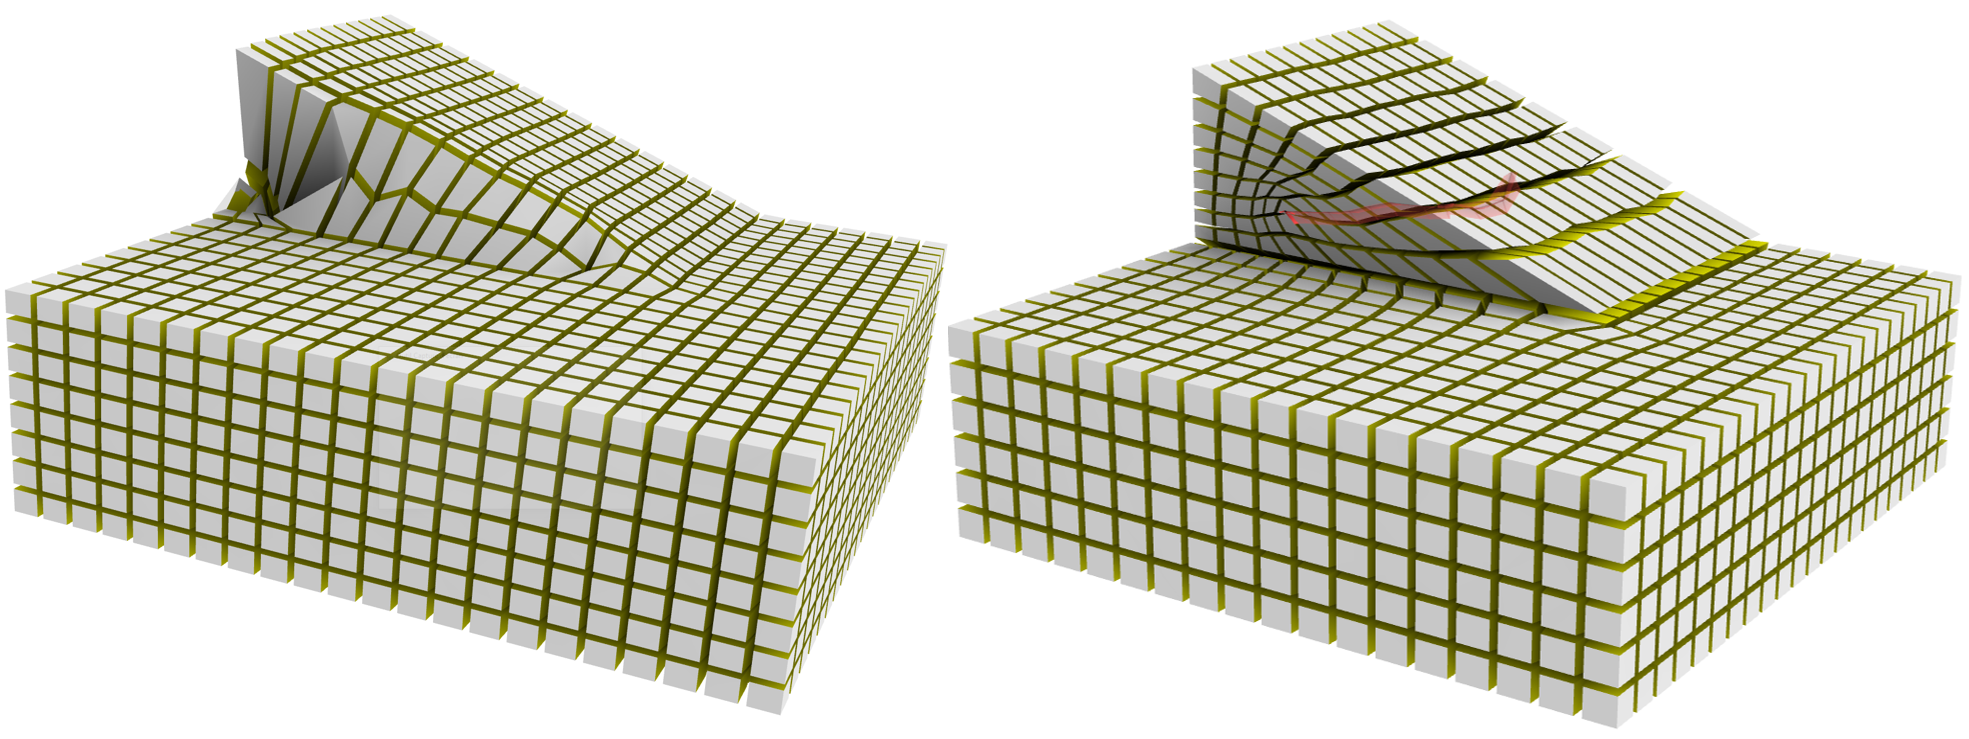
\includegraphics[width=0.8\textwidth]{img/hexmeshing_ff/tremplin_solved_2.PNG}
    \end{figure}
    
    Les champs de repère orthogonaux échouent lorsque l'angle de la pente est trop faible, donnant des résultats dégénérés (à gauche). En utilisant notre méthode, nous obtenons des contraintes de direction qui séparent correctement la pente et son support (à droite).
    
\end{frame}

\begin{frame}{Intuition de la méthode}

    \begin{figure}
        \centering
        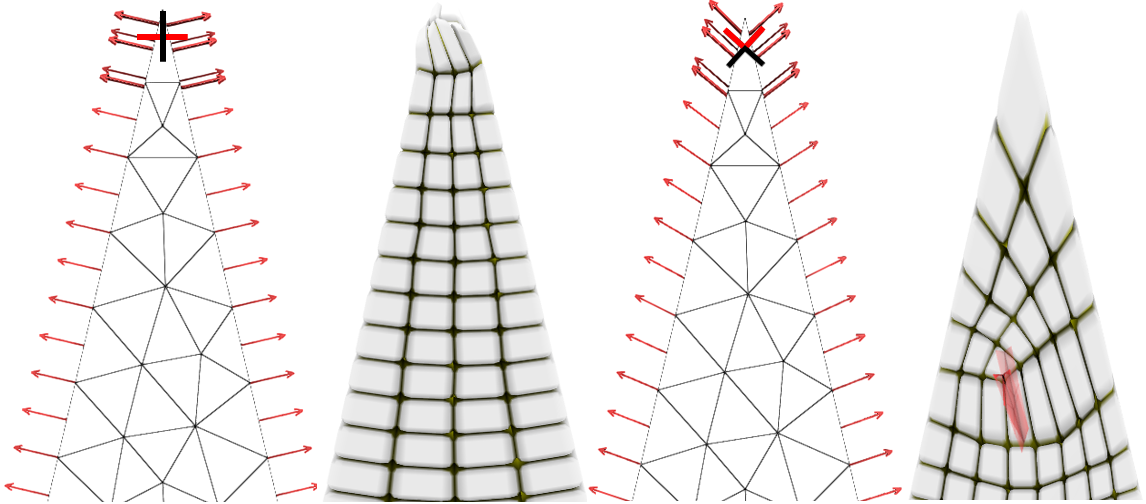
\includegraphics[width=0.8\textwidth]{img/hexmeshing_ff/normal_alignment_with_hexes_2.PNG}
    \end{figure}
    
    Un champ de repère orthogonal aligné avec les normales de surface peut créer une arête de valence 0 dans le cas d'une arête à petit angle (en haut à gauche), qui ne peut pas être maillée. En recalculant les contraintes de direction, nous obtenons une arête de valence 1 qui peut être maillée (en haut à droite).
    
\end{frame}

\begin{frame}{Calcul des angles dièdres et des valences géométriques}

    \begin{figure}
        \centering
        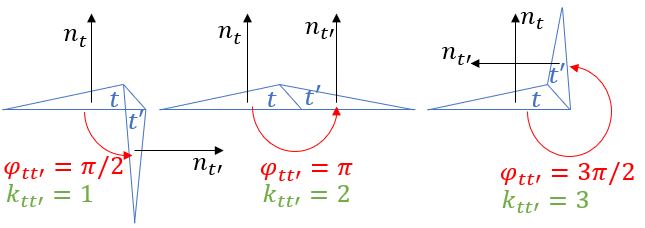
\includegraphics[width=0.8\textwidth]{img/hexmeshing_ff/phi_angles.PNG}
    \end{figure}
    
    \only<1-1>{
    L'angle dièdre $\varphi_{tt'}$ et la valence géométrique d'arête $k_{tt'}$ sont déterminés en utilisant les normales de faces $n_t$ et $n_{t'}$ adjacentes à l'arête de bord.
    }
    \only<2-2>{
        \begin{align*}
            \varphi(n_t, n_{t'}) &= \pi - \mathrm{atan2} \left( \langle n_t \times n_{t'}, \frac{e_{tt'}}{\left|e_{tt'}\right|} \rangle, \langle n_t , n_{t'} \rangle \right)\\
            k_{tt'} &= \text{arrondi}( \frac{\varphi_{tt'}}{\pi/2} )
        \end{align*}
    }
\end{frame}

\begin{frame}{Valences prescrites dans des modèles CAO}

    \begin{figure}
        \centering
        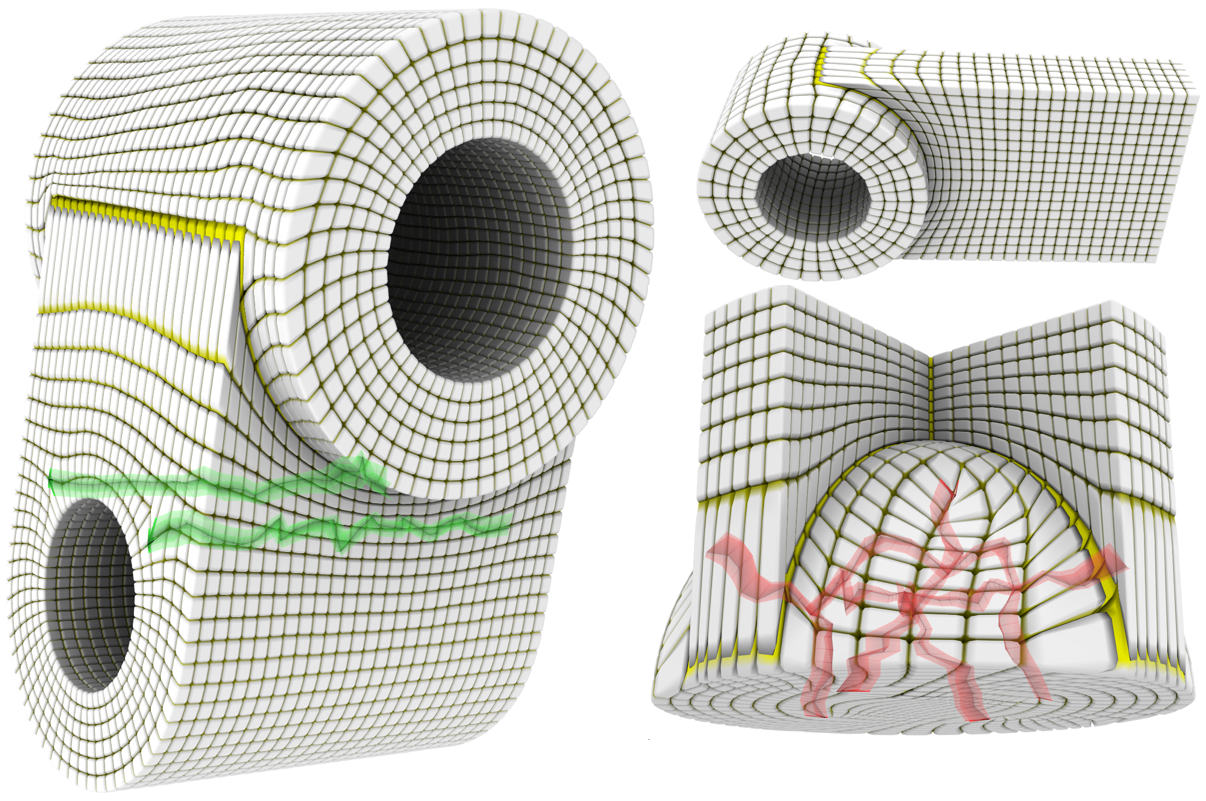
\includegraphics[width=0.7\textwidth]{img/hexmeshing_ff/prescribed_valences.PNG}
    \end{figure}
    
    \small
    Dans le cas de non-orthogonalité extrême dans des modèles CAO, il est difficile de déterminer géométriquement les valences des arêtes caractéristiques. Pour obtenir ces résultats, nous avons prescrit les valences des arêtes caractéristiques dans les descriptions CAO des modèles en entrée.
    
\end{frame}